
\documentclass[journal]{IEEEtran}

\usepackage[T1]{fontenc}

\usepackage{cite}
% cite.sty was written by Donald Arseneau
% V1.6 and later of IEEEtran pre-defines the format of the cite.sty package
% \cite{} output to follow that of IEEE. Loading the cite package will
% result in citation numbers being automatically sorted and properly
% "compressed/ranged". e.g., [1], [9], [2], [7], [5], [6] without using
% cite.sty will become [1], [2], [5]--[7], [9] using cite.sty. cite.sty's
% \cite will automatically add leading space, if needed. Use cite.sty's
% noadjust option (cite.sty V3.8 and later) if you want to turn this off
% such as if a citation ever needs to be enclosed in parenthesis.
% cite.sty is already installed on most LaTeX systems. Be sure and use
% version 4.0 (2003-05-27) and later if using hyperref.sty. cite.sty does
% not currently provide for hyperlinked citations.
% The latest version can be obtained at:
% http://www.ctan.org/tex-archive/macros/latex/contrib/cite/
% The documentation is contained in the cite.sty file itself.

% *** GRAPHICS RELATED PACKAGES ***
%
\ifCLASSINFOpdf
 \usepackage[pdftex]{graphicx}
  % declare the path(s) where your graphic files arest
  % \graphicspath{{../pdf/}{../jpeg/}}
  % and their extensions so you won't have to specify these with
  % every instance of \includegraphics
  \DeclareGraphicsExtensions{.pdf,.jpeg,.png,.eps}
\else
  % or other class option (dvipsone, dvipdf, if not using dvips). graphicx
  % will default to the driver specified in the system graphics.cfg if no
  % driver is specified.
  \usepackage[dvips]{graphicx}
  % declare the path(s) where your graphic files are
  % \graphicspath{{../eps/}}
  % and their extensions so you won't have to specify these with
  % every instance of \includegraphics
  \DeclareGraphicsExtensions{.eps}
\fi

% *** MATH PACKAGES ***
%
\usepackage[cmex10]{amsmath}
\usepackage{gensymb}

% *** ALIGNMENT PACKAGES ***
%
\usepackage{array}

% *** FLOAT PACKAGES ***
%
%\usepackage{fixltx2e}

\usepackage{stfloats}

\usepackage{multirow}

% \usepackage{dblfloatfix}

% *** PDF, URL AND HYPERLINK PACKAGES ***
%
\usepackage{url}

% correct bad hyphenation here
\hyphenation{op-tical net-works semi-conduc-tor}

\begin{document}

\title{Energy Resolution and Temperature Dependence of Ce:GAGG Coupled to 3mm $\times$ 3mm Silicon Photomultipliers}

\author{B.~Seitz, 
	N.~Campos~Rivera
	and~A.~G.~Stewart% <-this % stops a space

\thanks{B.~Seitz and N.~Campos~Rivera are with the Scottish Universities Physics Alliance (SUPA), School of Physics and Astronomy, University of Glasgow, Glasgow, G12 8QQ, Scotland, UK (email: bjoern.seitz@glasgow.ac.uk). \mbox{A. G. Stewart} was with the SUPA School of Physics and Astronomy, University of Glasgow. He is now with the Industrial Biotechnology Innovation Centre (IBioIC), Glasgow, UK, G1 1RD. (email: andrew.stewart@ibioic.com)}% <-this % stops a space
\thanks{Manuscript received July xx, 2015; revised X xx, 2015.}}

\markboth{IEEE TRANSACTIONS ON NUCLEAR SCIENCE,~Vol.~XX, No.~X, XXXX~2015}%
{Shell \MakeLowercase{\textit{et al.}}: Bare Demo of IEEEtran.cls for Journals}

% make the title area
\maketitle

\begin{abstract}
Scintillators are a critical component of sensor systems for the detection of ionizing radiation. Such systems have a diverse portfolio of applications from medical imaging, well logging in oil exploration and detection systems for the prevention of the illicit movement of nuclear materials. The rare earth element cerium is an ideal dopant for a variety of host scintillating materials due to the fast 5d$_{1}$ $\rightarrow$ 4f radiative transition of Ce$^{3+}$. Cerium-doped Gadolinium Aluminium Gallium Garnet (Ce:GAGG) is a relatively new single crystal scintillator with several interesting properties. These include high light yield; an emission peak well-matched to silicon sensors; and a low intrinsic energy resolution. Moreover, the material has a high density and is non-hygroscopic. In this article we review the properties of cerium-doped GAGG and report energy resolution measurements over the temperature range -10\celsius{} to +50\celsius{} for 3 $\times$ 3 $\times$ 30 mm$^{3}$ Ce:GAGG crystals optically coupled to a Silicon Photomultipler (SiPM) sensor with a 3mm $\times$ 3mm active area. In addition the linearity of the scintillator-SiPM response as a function of gamma energy is reported. 
\end{abstract}

% Note that keywords are not normally used for peerreview papers.
\begin{IEEEkeywords}
Scintillation Detection, Ce:GAGG, Silicon Photomultiplier, Gamma Spectroscopy, Positron Emission Tomography, PET.
\end{IEEEkeywords}

\section{Introduction}
\IEEEPARstart{C}{erium}-doped Gd$_{3}$Al$_{2}$Ga$_{3}$O$_{12}$ (Ce:GAGG) is a relatively new single crystal scintillator with several properties that make it interesting for applications such as gamma spectroscopy \cite{gamma:iwan, gagg:orita}, alpha particle detection \cite{alpha:morishita, sipm:morishita} and nuclear medicine \cite{gagg:levin, gagg:seitz, gagg:fbk, gagg:schneider, gagg:kamada04}. The material was first reported in 2011 and single crystals can be grown by the Czochralski (Cz) method \cite{gagg:kamada01, gagg:kamada02}. It is the brightest of the oxide scintillators with a Light Yield (LY) of 46,000 photons/MeV and an emission peak at 530nm from the 5d $\rightarrow$ 4f radiative transition. 

GAGG has no intrinsic radioactivity and is non-hygroscopic. The crystal has been studied as a suitable scintillator for the block detectors used in Positron Emission Tomography (PET) and Single Photon Emission Tomography (SPECT) scanners. The crystal is mechanically stable and crystals with dimensions as small as 0.4mm $\times$ 0.4mm $\times$ 5mm have been reported for use in ultra-high resolution block detectors \cite{yamamoto:ultrahigh}.  


\begin{table}[bt]
\renewcommand{\arraystretch}{1.3}
\caption{Review of Properties of Ce:GAGG}
\label{tab:gagg_review}
\centering
\begin{tabular}{ c | c | c | c | c | c }
\hline
\bfseries Crystal Size & \bfseries Ce & \bfseries LY & \bfseries ER & \bfseries Decay & \bfseries Ref \\
\bfseries (mm) & \bfseries (\%) & \bfseries (ph/MeV) & \bfseries (\%) & \bfseries (ns) & \\
\hline \hline
3 $\phi{} \times{}$ 1 ($\mu$PD) & 0.2 & 42,000 & 8.3 & 53.7 &\cite{kamada:sc_scint} \\
\hline
5 $\times$ 5 $\times$ 1 & 1 & 46,000 & 4.9 & 88 & \cite{gagg:kamada02} \\
\hline
3 $\times$ 3 $\times$ 1 & 1 & 46,000 & 7.8 & 92 & \cite{gagg:kamada03} \\
\hline
5 $\times$ 5 $\times$ 1 & 1 & 47,900 & 6.8$\pm{}$0.2 & - & \cite{sakthong:gagg} \\
\hline
10 $\times$ 10 $\times$ 5 & - & 33,000 & 5.2 & 127$\pm$6 & \cite{gamma:iwan} \\
\hline 
5 $\times$ 5 $\times$ 1 & 1 & 50,600 & 5.5 & - &\\
5 $\times$ 5 $\times$ 10 & 1 & 41,100 & 7.3 & - & \cite{prusa:lightyeild} \\
\hline
\end{tabular}
\end{table} 

\section{Review of Properties}

The usual figure-of-merit values from recent studies of Ce:GAGG are summarized in table~\ref{tab:gagg_review}. All the samples detailed in the table were grown by the Cz method except for the first one which was grown by the micropull-down method ($\mu$PD).

\subsection{Light Yield}
The LY, typically measured in response to 662keV gamma photons, has been reported to be as high as 50,600 photons per MeV \cite{prusa:lightyeild} and has been found to decrease with sample thickness \cite{prusa:lightyeild, sakthong:gagg} and Ce dopant concentration \cite{gagg:kamada03, prusa:lightyeild, Kamada:ce_conc, gagg:drozdowski}. The dependence on sample thickness is the result of the loss of photons due to self-absorption and scattering while the reduction in LY with increasing Ce content is attributed to Ce aggregate centres or crystal defects resulting from localized concentrations of Ce. 
The LY of Ce:GAGG is approximately 43\% higher than for cerium-doped lutetium-yttrium orthosilicate (Ce:LYSO), the established standard scintillator for PET. A ceramic version of the Ce:GAGG scintillator, produced by sintering crystalline nano-micrograins into a bulk ceramic, has also been reported. The ceramic version of the scintillator is reported to have a LY of 70,000ph/MeV \cite{yan:gagg}. 
  
\subsection{Intrinsic Energy Resolution}

The ER of a photopeak or full energy peak is defined as the Full Width Half Maximum (FWHM) of the peak divided by the mean value and when measured by coupling a scintillator to a detector, such as a PhotoMultiplier Tube (PMT), can be written as,
\begin{equation}
(\Delta{}E/E)^{2} = (\delta{}_{sc})^{2} + (\delta{}_{p})^{2} + (\delta{}_{st})^{2}
\end{equation}
\noindent{}where $\delta_{sc}$ is the intrinsic energy resolution of the crystal, $\delta{}_{p}$ is the transfer resolution, $\delta_{st}$ is the resolution of the detector and $\Delta{}E/E$ is the energy resolution of the scintillation-sensor system. The main contribution to the intrinsic resolution of the crystal is the non-proportionality in the number of soft photons generated as a function of gamma energy. The non-proportionality of Ce:GAGG has been studied by a number of groups and is of the order of 20\% over the energy range 32 to 662keV. The intrinsic ER of single crystal Ce:GAGG at a gamma energy of 662keV is in the range 4.9-7.8\%. At the lower end of this range, the energy resolution is a factor of 1.6 better than Ce:LYSO ($\sim$8\%) and similar to that of thallium-doped cesium iodide (Tl:CsI).   

\subsection{Decay Time}

The decay of the scintillation light pulse is reported to have two components; a fast component of the order of 60-130ns and a slow component of the order of several hundred nanoseconds (260-530ns). In the lower range of the fast component, the decay time is comparable to the radiative lifetime of Ce$^{3+}$ \cite{kamada:sc_scint}. The decay time as a function of Ce concentration has been studied and found to decrease with increasing concentration \cite{gagg:kamada03}. The pulse decay time in the transparent ceramic version of Ce:GAGG is reported to be 165ns \cite{yan:gagg}. 

\section{Experimental}

% figure 1
\begin{figure}[tb]																			
\centering
\includegraphics[width=3in]{gagg_crystals.jpg}
\caption{3mm $\times$ 3mm $\times$ 30mm Ce:GAGG crystals from Furukawa Co. Ltd. Japan. The crytals were polished on all faces and 5 faces were covered with a white reflective coating.}
\label{fig:GAGG}
\end{figure}

%\subsection{Scintillating Crystals for Medical Imaging}
%
%
\subsection{Cerium doped Gd$_{3}$Al$_{2}$Ga$_{3}$O$_{12}$ (Ce:GAGG)}
The properties of Ce:GAGG samples used in this study are summarized in table~\ref{tab:scint_properties}. For comparison the properties of thallium-doped sodium iodide (Tl:NaI) and the oxide scintillators Bi$_{4}$Ge$_{3}$O$_{12}$ (BGO) and Ce:LYSO are also given. Tl:NaI is one of the most widely used scintillating materials while BGO was the material of choice for early positron emission tomography scanners. Modern PET systems use Ce:LYSO. The crystals used in this study have dimensions 3 $\times$ 3 $\times$ 30 mm$^{3}$ and were supplied by Furukawa Co. Ltd, Japan. All faces of the crystals had been polished and 5 faces were coated in a white reflective material. A photograph of the four crystals are shown in figure \ref{fig:GAGG}. 
%
\subsection{Silicon Photomultiplier Sensor Platform}
The Silicon Photomultiplier sensor platform consists of a 2D array of microcells \cite{sipm:saveliev, sipm:stewart}. Each microcell is composed of a photon counting or Geiger-mode Avalanche Photodiode (GAPD) in series with a passive quenching element. For each detected photon the microcell emits a pulse of current and is considered a digital device \cite{stew02:stewart}. However, as all the microcells are connected in parallel to a single output, the summed output forms an analogue output in which the total emitted charge is proportional to the number of incident photons detected. 

The SiPM is an ideal sensor for the optical read-out of scintillating materials and its compact size and form factor allow for the design of highly granular detectors with one-to-one coupling between the scintillator and the sensor. Additional benefits of the SiPM platform include ease of operation, inherent immunity to interference by strong magnetic fields and a low operating voltage. Another key feature of the platform is its compatibility with modern semiconductor manufacturing processes (CMOS) which allows the sensors and processing electronics to be combined on a single chip. 

\begin{table}[bt]
\renewcommand{\arraystretch}{1.3}
\caption{Properties of Scintillating Materials}
\label{tab:scint_properties}
\centering
\begin{tabular}{l | c | c | c | c }
\hline
\bfseries  & \bfseries Ce:GAGG & \bfseries Ce:LYSO & \bfseries BGO & \bfseries Tl:NaI \\
\hline \hline
Light Yield [photons/MeV] & 46,000 & 32,000 & 8,000 & 40,000\\
Decay Time [ns] & 90 & 41 & 300 & 230\\
Peak Emission [nm] & 520 & 420 & 480 & 415\\
Density [g/cm$\textsuperscript{3}$] & 6.6 & 7.1 & 7.13 & 3.67\\
Intrinsic ER [\%] & 5.2 & 8 & 12 & 6.6\\
Z$_{\text{eff}}$  & 54 & 66 & 75 & 51\\
\hline
\end{tabular}
\end{table}

\begin{table}[t] % Table III
\renewcommand{\arraystretch}{1.2}
\caption{SiPM Sensor Parameters}
\label{tab:spm_param}
\centering
\begin{tabular}{l | c }
\hline
\bfseries Parameter &  \bfseries SiPM\\
\hline \hline
Structure & P-on-N\\
Active Area (mm) & 3 $\times$ 3\\
Microcell Dimensions ($\mu$m) & 35 $\times$ 35\\
Number of Microcells & 4774\\
Fill Factor & 64\%\\
Breakdown Voltage (20\celsius{}) & 24.7V\\
Peak Response ($\lambda$) & 420nm\\ 
PDE at peak $\lambda$ (V$_{\text{br}}+2.5V$) & 31\%\\
\hline
\end{tabular}
\end{table}

%
\subsection{Experimental Setup}

To provide a dark, temperature-controlled environment, the scintillator-SiPM detector, amplifier and radioactive source were placed inside a Heraeus Votsch 4004 environmental chamber. The chamber was used to vary the temperature of the scintillator-SiPM detector between -10 and +50\celsius{}. Optical coupling between the uncoated scintillator facet and the SiPM sensor was achieved using Dow Corning 20-057 (n = 1.48) optical coupling compound. 

The SiPM used in this study was a 3mm $\times$ 3mm MicroFC sensor from SensL \cite{sensl:oneill2}. While the MicroFC is not the best spectral match to Ce:GAGG, the peak optical response of the MicroFC occurs at 420nm compared with the emission peak of 520nm for Ce:GAGG, the device has significantly lower noise performance (dark rate) than similar devices with peak sensitivity in the green \cite{stewart:microFC}. The MicroFM has a peak response of 500nm and is therefore a better spectral match to Ce:GAGG. The MicroFC consists of 4774 microcells and has a fill factor of 64\%. The main features of this sensor are summarized in table~\ref{tab:spm_param}.  

The SiPM signal was amplified using a high bandwidth amplifier from MiniCircuits. The amplified signals were displayed on a 1GHz LeCroy (LC574AL) oscilloscope. The detected signals were captured and transferred from the oscilloscope to a PC for further processing. The amplitude of each signal pulse was taken as a measure of the energy deposited by the gamma photon inside the crystal. A minimum of 10,00 pulses was used to generate the pulse height spectrum for each gamma energy.  

\section{Experimental Results}

\subsection{IV Characteristics}

Figure~\ref{fig:iv} shows the reverse bias portion of the IV characteristic of a 3mm $\times$ 3mm MicroFC sensor recorded at 20\celsius{} and -10\celsius{}. The IV characteristic was used to determine the temperature dependence of the junction breakdown voltage and was recorded at several temperatures between -10 and 20\celsius{}. Figure~\ref{fig:IVT} shows the  breakdown voltage as a function of temperature. The breakdown voltage decreases monotonically with decreasing temperature and has a temperature coefficient of 20mV/\celsius{}. 

%figure 2
\begin{figure}[tb]
\centering
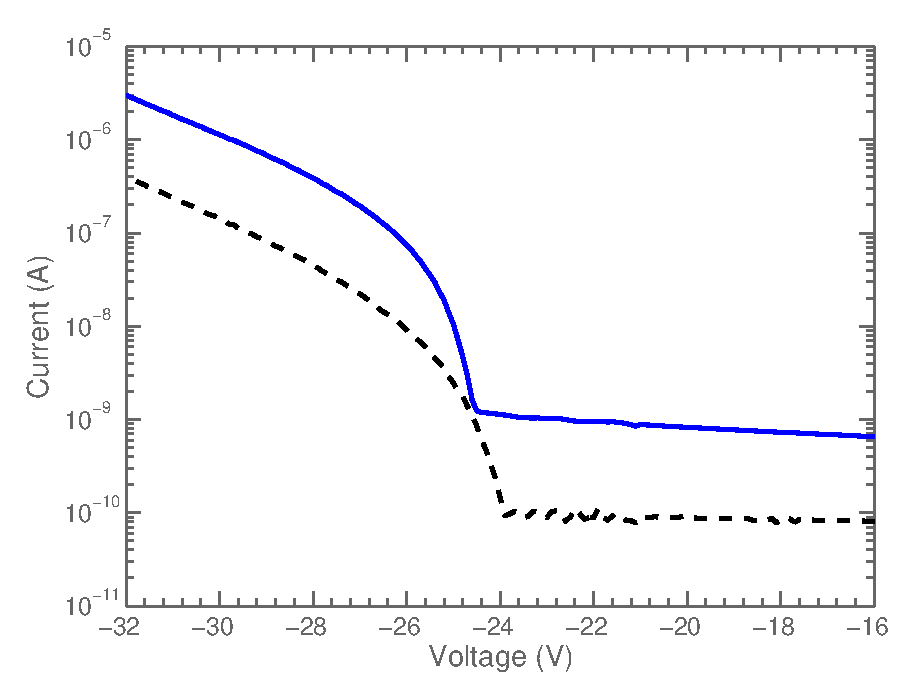
\includegraphics[width=3in]{fig1_IV.eps}
\caption{Current-Voltage Characteristics of 3mm  measured at 20\celsius{} (solid blue curve) and -10\celsius{} (dashed black curve).}
\label{fig:iv}
\end{figure}

%figure 3
\begin{figure}[tb]
\centering
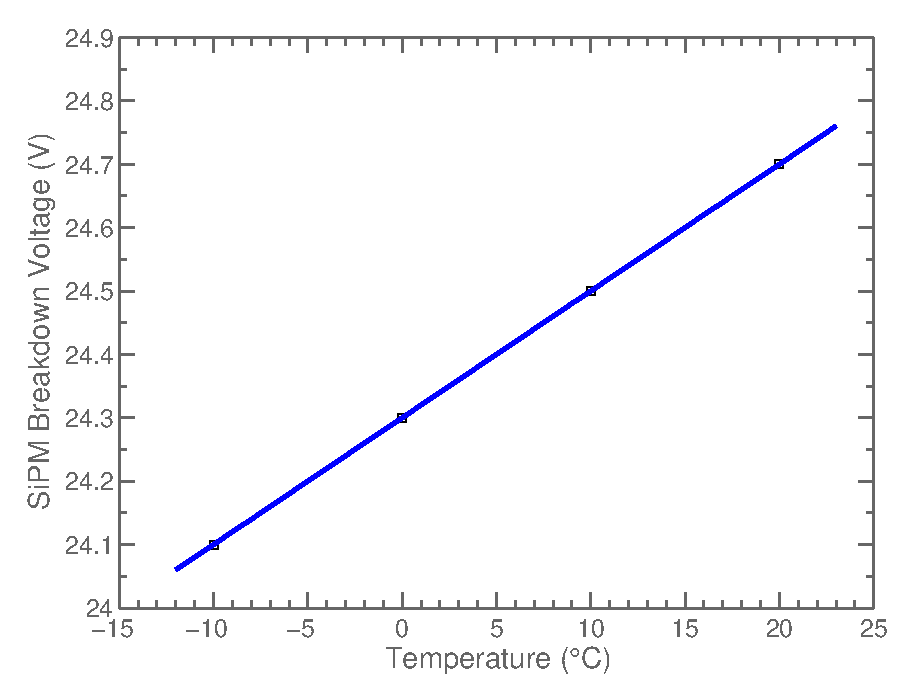
\includegraphics[width=3in]{vbr_temp_depend.eps}
\caption{Temperature dependence of the SiPM breakdown voltage. The device breakdown voltage has a temperature coefficient of 20mV/\celsius{}.}
\label{fig:IVT}
\end{figure}

\subsection{Detector Response Linearity}
As described above, a silicon photomultiplier consists of a limited number of single-photon sensitive microcells. The detection of a photon, assuming a uniform spatial distribution, is a statistical process based on the probability that the photon is absorbed within the sensitive volume of a microcell and the probability that the photo-generated electron or hole initiate an avalanche breakdown of the GAPD \cite{geiger:mcintyre}. In addition, the mircocells have a finite recovery time during which the microcells can be considered insensitive to photons. The dynamic range of an SiPM is therefore a function of the number of microcells and the sensor Photon Detection Efficiency (PDE). For an instantaneous light pulse, the number of detected photons can be approximated by the expression,
\begin{equation} \label{first}
N_{d} = N_{MC}\cdot{}(1 - exp(-\frac{\eta{}\cdot{}N_{ph}}{N_{MC}}))
\end{equation}
where $N_{d}$ is the number of detected photons, $N_{ph}$ is the number of incident photons, $\eta$ is the SiPM PDE, and $N_{MC}$ is the total number of microcells. This expression gives an approximately linear response when the number of detected photons ($\eta{}\times{}N_{ph}$) is much less than the total number of microcells ($N_{MC}$). However, the response begins to saturate as the number of detected photons approaches the number of microcells. Hence there is a trade-off between the geometry, the dimensions and number of microcells for a given area, the PDE and the dynamic range. A more complex model of the response of an SiPM sensor that takes into account the effects of the recovery time, afterpulsing and crosstalk has also been developed \cite{model:dam}.

Figure~\ref{fig:saturation} shows the photopeak mean height as a function of gamma energy at 2, 3, 4 and 5V above the SiPM breakdown voltage. The measurements were recorded at 20\celsius{} using $^{241}$Am, $^{133}$Ba and $^{137}$Cs sources. At 2 and 3V above the breakdown voltage, the response shows good linearity with increasing gamma energy. At 4 and 5V above the breakdown voltage the data sets are fitted with an exponential saturation model. In addition, the gamma energies between 60keV and 356keV are fitted with a linear model which is extrapolated to 680keV to show the deviation from linearity. At 5V above the breakdown voltage and at 662keV the response of the detector is approximately 6.5\% below that expected from a linear trend. 

% figure 4
\begin{figure}[tb]
\centering
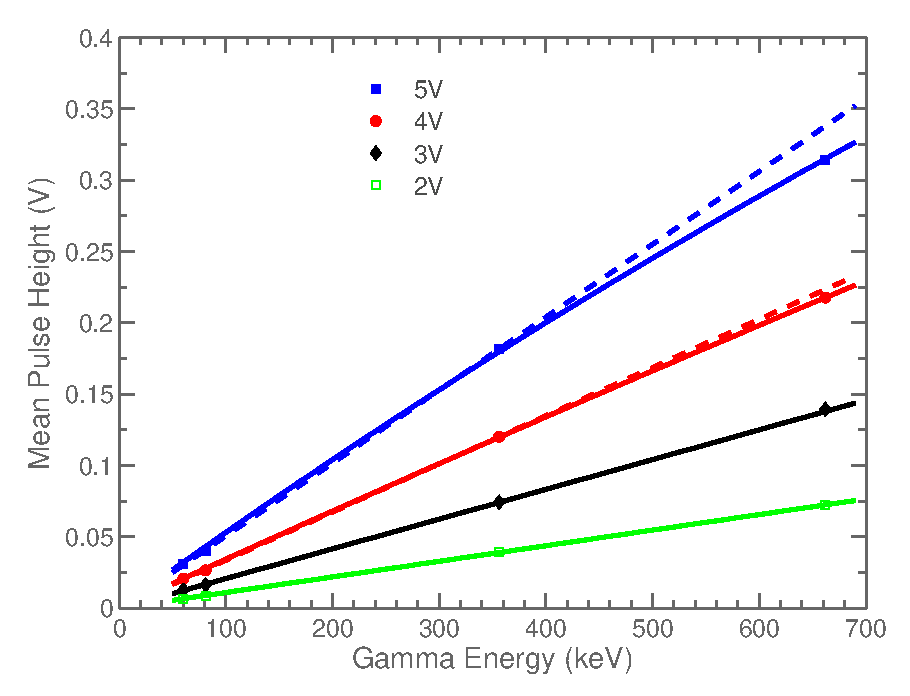
\includegraphics[width=3in]{sat_curves.eps}
\caption{Photopeak mean height as a function of gamma energy for Ce:GAGG optically coupled to the SiPM sensor at 20\celsius{}. The data shows the mean pulse height at SiPM bias values of 2V (green squares), 3V (black diamonds), 4V (red circles) and 5V (blue squares) over the breakdown voltage. The data at 4 and 5V above the breakdown voltage are fitted with an exponential saturation curve (equation~\ref{first}) and a linear model (excluding the 662keV data point) to show the deviation from linearity at higher energies.}
\label{fig:saturation}
\end{figure}


\subsection{Pulse Decay Time}
Figure~\ref{fig:decay} shows the decay time of the scintillation pulse from 662keV gamma photons at 20\celsius{}. The pulse shape was averaged for 2000 pulses using the oscilloscope   and transferred to a PC for analysis. The decay time was obtained by fitting the pulse with a single exponential with a decay constant, $\tau$, of 191ns. 

% figure 5
\begin{figure}[tb]
\centering
\includegraphics[width=3in]{decay_curve_rt.eps}
\caption{Pulse shape from Ce:GAGG-SiPM detector in response to 662keV gamma photons. The data represents the average shape from 2000 pulses. The pulse decay is fitted with a single exponential decay (red dashed curve) with a decay constant, $\tau$, of 191ns. }
\label{fig:decay}
\end{figure}

\subsection{Energy Resolution}

Figure~\ref{fig:er} shows the pulse height spectrum for the scintillator-SiPM detector in response to 662keV gamma photons ($^{137}$Cs) at 20\celsius{}. The spectrum is modeled as the sum of two Gaussian distributions; one fitted to the Compton edge of the spectrum and one fitted to the photopeak. The energy resolution is defined as the FWHM divided by the centroid of the Gaussian fit to the photopeak. The 662keV photopeak in figure~\ref{fig:er} has an energy resolution of 10.2$\pm$0.5\%. After correcting for the saturation effect, described in section B, the energy resolution is 10.5\%.  

\subsection{Bias Dependence}
The energy resolution as a function of SiPM bias is shown in figure ~\ref{fig:erbias}. The figure shows the energy resolution for 662eV gamma photons as a function of SiPM bias recorded at 20\celsius{}. Both the uncorrected and corrected energy resolution values are displayed. The corrected values were determined by measuring the SiPM response, as described in section B, at each bias value. At high bias values, the figure shows that the energy resolution (corrected) begins to saturate at about 4V above the breakdown voltage. 

The SiPM PDE, gain and noise (dark rate, cross-talk and after-pulsing) are all functions of the applied bias and the relationship between these terms and the bias determines the bias dependence of the energy resolution. For relatively large optical signals, such as those for high LY scintillators, the bias dependence of the PDE largely determines the response of the energy resolution. As a function of the applied bias, the PDE initially increases rapidly resulting in a reduction in the energy resolution as the photopeak mean increases faster than the variance. As the bias dependence of the PDE begins to level-off, the energy resolution also begins to saturate assuming that the SiPM response is operating in the linear region of its response. 

\subsection{Temperature Dependence}
The temperature dependence of the energy resolution measured at 662keV and at a constant overbias of 4V above the breakdown voltage is shown in figure~\ref{fig:ertemp}. The energy resolution values are uncorrected for the effect of saturation of the SiPM response and the y errorbars are calculated from the one sigma confidence intervals from the FWHM and centroid parameters of the Gaussian fit. At 662keV the main contribution to the energy resolution comes from the intrinsic energy resolution of the crystal since the large number of soft photons produced far exceeds the SiPM noise (dark rate) and contribution from photon statistics. 

Figure~\ref{fig:photopeak_temp} shows the 662keV photopeak mean, measured at both a constant overbias (4V above the breakdown voltage) and a constant bias, as function a temperature. At a fixed bias the photopeak mean decreases approximately linearly with increasing temperature. This is a direct result of the temperature dependence of the breakdown voltage of the SiPM and the resulting reduction in the sensor overbias. As the sensor overbias is reduced, the PDE and gain of the sensor decrease and hence the photopeak mean decreases. For a fixed overbias, the photopeak mean is relatively constant over the temperature range -10\celsius{} to 30\celsius{}. Above 30\celsius{}, the photopeak mean was observed to decrease by 10.6\% between 30\celsius{} and 50\celsius{}. This temperature dependence is similar to that reported in \cite{temp:yan}. This reduction is likely to be the result of thermal quenching of the radiative transition in Ce$^{3+}$. 

% figure 6
\begin{figure}[t]
\centering
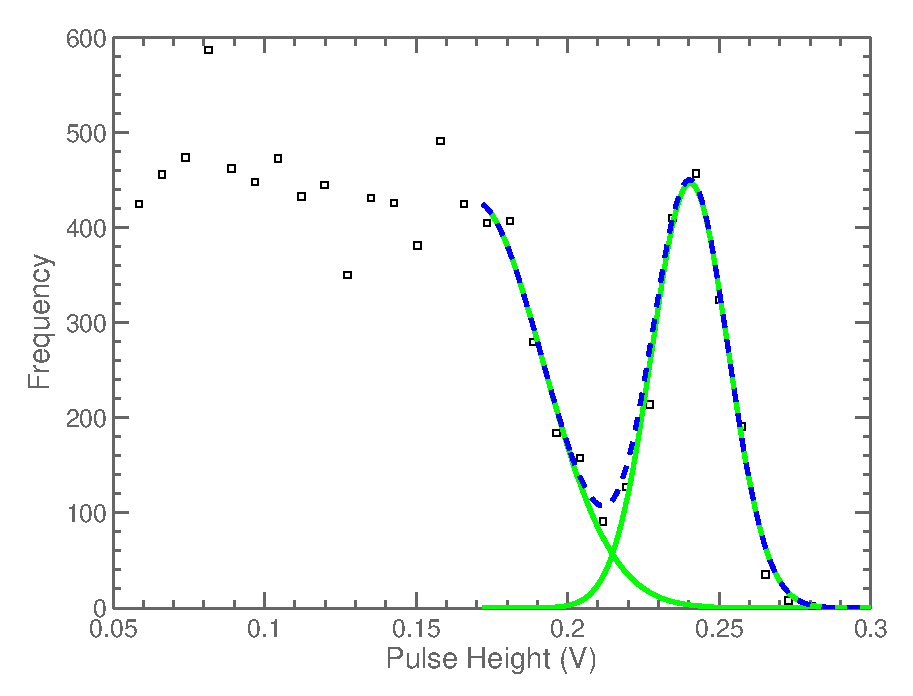
\includegraphics[width=3in]{energy_resolution.eps}
\caption{Pulse height spectrum for a 3 $\times$ 3 $\times$ 30 mm$^{3}$ Ce:GAGG crystal coupled to a 3 mm $\times$ 3 mm SiPM recorded at room temperature (20\celsius{}). The 662keV ($^{137}$Cs) photopeak has a saturation corrected energy resolution of 10.5$\pm$0.5\%. The detector bias was 28.7V or 4V above the breakdown voltage.}
\label{fig:er}
\end{figure}

%figure 7
\begin{figure}[tb]
\centering
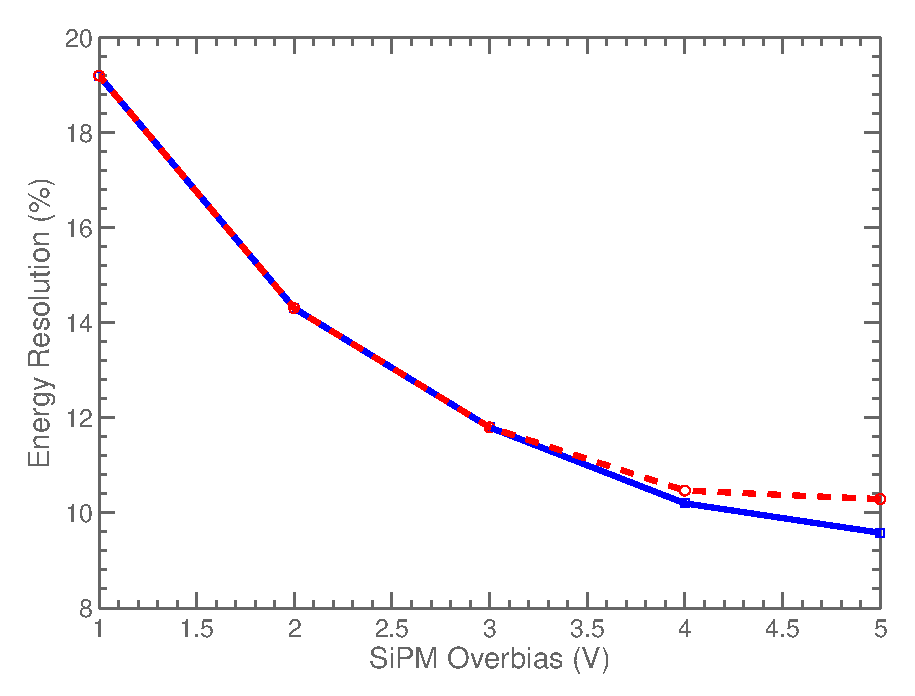
\includegraphics[width=3in]{er_obias.eps}
\caption{Energy Resolution for 662keV ($^{\text{137}}$Cs) gamma photons as a function of SiPM bias measured at 20\celsius{}. The blue squares represent the uncorrected measured values while the red circles represent the data after correction for saturation (see figure~\ref{fig:saturation}).}
\label{fig:erbias}
\end{figure}

%figure 8
\begin{figure}[tb]
\centering
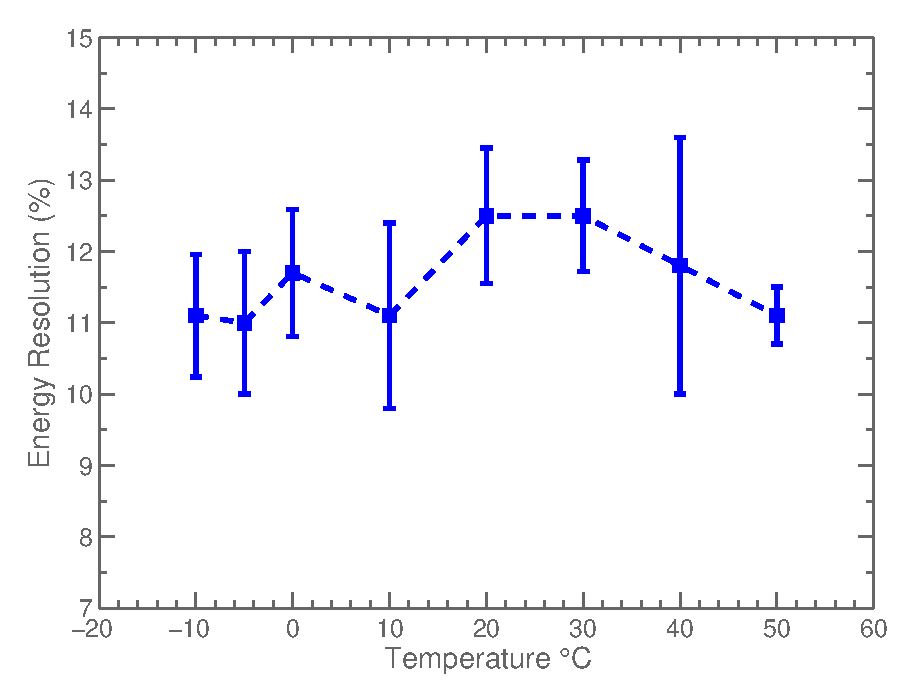
\includegraphics[width=3in]{temp_er.eps}
\caption{Energy Resolution at 662keV as a function of temperature. The pulse height spectrum was recorded at each temperature for a constant over-bias of 4V above the break-down voltage. The energy resolution values are uncorrected for the effect of saturation of the SiPM response. The data points are joined by a dashed line as a guide for the eye.}
\label{fig:ertemp}
\end{figure}

%figure 9
\begin{figure}[tb]
\centering
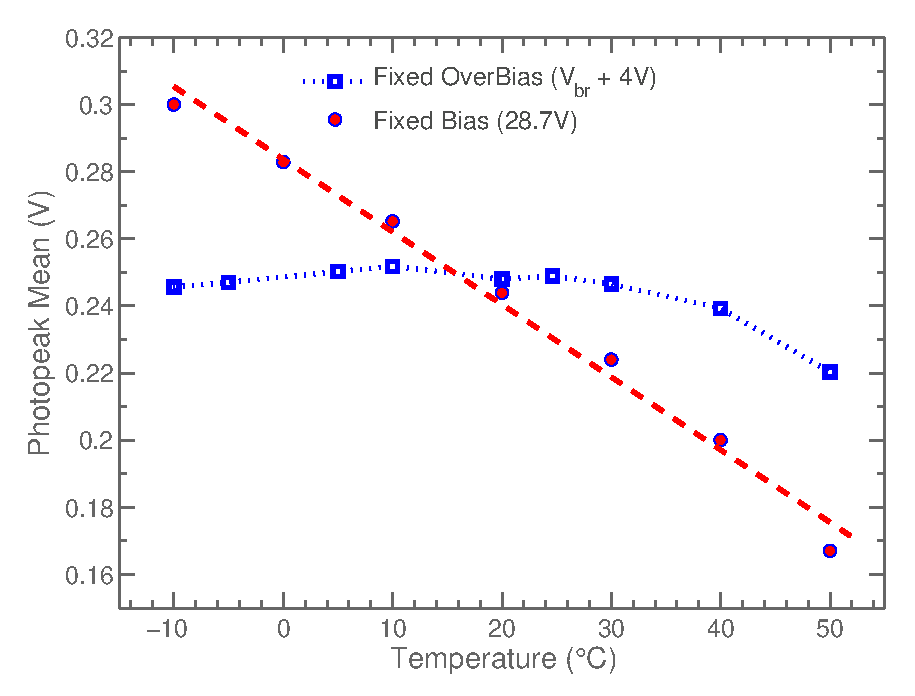
\includegraphics[width=3in]{temp_depend_all.eps}
\caption{Photopeak mean as a function of temperature. The data points are joined by a dotted line as a guide for the eye.}
\label{fig:photopeak_temp}
\end{figure}

%figure 10
%\begin{figure}[tb]
%\centering
%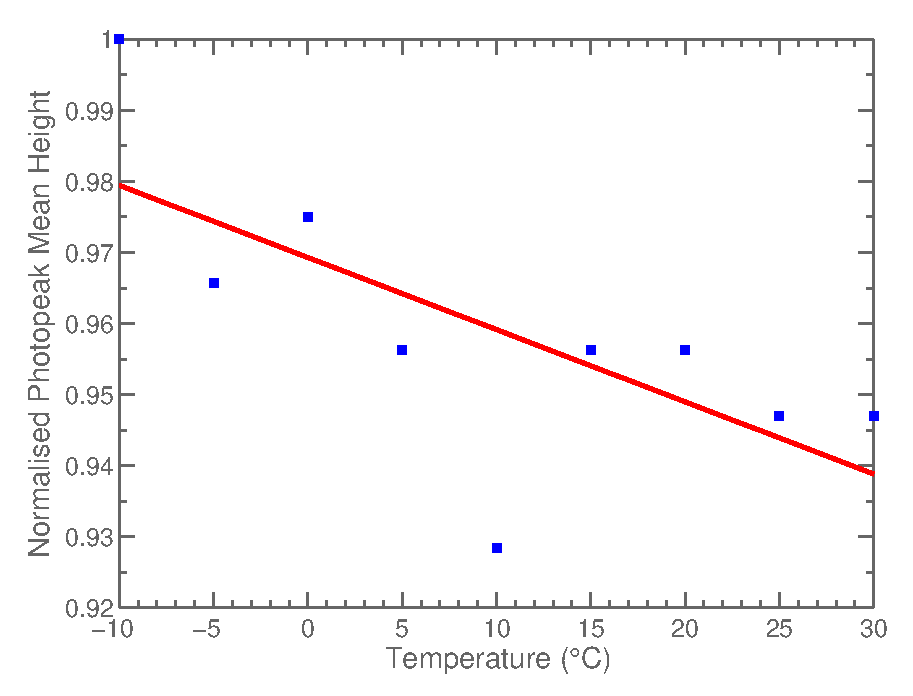
\includegraphics[width=3in]{temp_depend.eps}
%\caption{Temperature dependence}
%\label{fig:temp_depend}
%\end{figure}

% \appendices
%\section{Proof of the First Zonklar Equation}
% Appendix one text goes here.

%\section{}
%Appendix two text goes here.


\section{Discussion}

Cerium-doped GAGG has a high light yield and excellent intrinsic energy resolution that make it a promising scintillator material for a range of applications including medical imaging. With minimal optimization, an energy resolution of 10.5\% was achieved when optically coupled to a 3mm $\times$ 3mm SiPM sensor at room temperature. Below 30\celsius{} the light output of scintillator is relatively constant while above 30\celsius{} the thermal quenching of the Ce$^{3+}$ transition was observed.  

While the light yield and intrinsic energy resolution of Ce:GAGG is superior to Ce:LYSO, the longer decay time and lower atomic number remains a drawback for the adoption of the Ce:GAGG in modern PET scanners. The lower atomic number results in a reduced gamma detection efficiency and hence a longer scan time would be required to generate the required statistics compared with Ce:LYSO crystals with similar axial dimensions. The longer decay time increases the probability of pile-up effects.

\section{Conclusion}

Cerium-doped GAGG is a promising scintillating crystal for a number of applications including medical imaging modalities such as PET and SPECT. The crystal has the highest LY of the oxide scintillators, a low intrinsic energy resolution and relatively fast timing properties. A room temperature energy resolution, corrected for the effect of saturation, of 10.5\% was recorded for a 3 $\times$ 3 $\times$ 30 mm$^{3}$ crystal coupled to a 3 $\times$ 3 mm$^{2}$ SiPM sensor. The energy resolution shows an improvement at lower temperatures while the mean of the photopeak was observed to decrease at temperatures greater than 30\celsius{}.


\section*{Acknowledgement}
%
Dr Stewart was supported by a fellowship from the \mbox{Scottish} Universities Physics Alliance (SUPA). This work has been partially supported by the European Union Framework 7 Project HadronPhysics3 (FP7 Project Ref: 283286). The authors acknowledge and thank Carl Jackson, Liam Wall and Kevin O'Neill at SensL for assistance with the SiPM sensors. 

% Can use something like this to put references on a page
% by themselves when using endfloat and the captionsoff option.
\ifCLASSOPTIONcaptionsoff
  \newpage
\fi

\begin{thebibliography}{1}

%1
\bibitem{gamma:iwan}
J.~Iwanowska, L.~Swiderski, T.~Szczesniak, P.~Sibczynski, M.~Moszynski, M.~Grodzicka, K.~Kamada, K.~Tsutsumi, Y.~Usuki, T.~Yanagida, ``Performance of cerium-doped Gd$_{3}$Al$_{2}$Ga$_{3}$O$_{12}$ (GAGG:Ce) scintillator in gamma-ray spectrometry'', \emph{Nucl. Instrum. Meth. A}, vol. 712, pp. 34-40, 2013.

%2
\bibitem{gagg:orita}
T.~Orita, K.~Shimazoe, H.~Takahashi, ``The dynamic time-over-threshold method for multi-channel APD based gamma-ray detectors'', Nucl. Instrum. Meth. A, vol. 775, pp. 154-161, 2015. 

%3
\bibitem{alpha:morishita}
Y.~Morishita, S.~Yamamoto, K.~Izaki, J.~H.~Kaneko, K.~Toui, Y.~Tsubota, M.~Higuchi, ``Performance comparison of scintillators for alpha particle detectors'', Nucl. Instrum. Meth. A, 764, pp. 383-386, 2014. 

%4
\bibitem{sipm:morishita}
Y.~Morishita, S.~Yamamoto, K.~Izaki, J.~H.~Kaneko, K.~Toi, Y.~Tsubota, ``Development of a Si-PM based alpha camera for plutonium detection in nuclear fuel facilities'', \emph{Nucl. Instrum. Meth. A}, vol. 747, pp. 81-86, 2014.

%5
\bibitem{gagg:seitz}
B.~Seitz, A.~G.~Stewart, K.~O'Neill, L.~Wall, C.~Jackson, ``Performance evaluation of novel SiPM for medical imaging applications'', \emph{Proc. IEEE Nucl. Sci. Symp. Conf. Rec.}, 2013. 

%6
\bibitem{gagg:levin}
J.~Y.~Yeom, S.~Yamamoto, S.~E.~Derenzo, V.~Ch.~Spanoudaki, K.~Kamada, T.~Endo, C.~S.~Levin, ``First Performance Results of Ce:GAGG Scintillation Crystals with Silicon Photomultipliers'', \emph{IEEE Trans. Nucl. Sci.}, vol. 60, no. 2, pp. 988-992 April 2013.

%7
\bibitem{gagg:fbk}
A.~Ferri, A.~Gola, N.~Serra, A.~Tarolli, N.~Zorzi, C.~Piemonte, ``Performance of FBK high-density SiPM technology coupled to Ce:LYSO and Ce:GAGG for TOF-PET'', \emph{Phys. Med. Biol.} vol. 59, pp. 869-880, 2014

%8
\bibitem{gagg:schneider}
F.~R.~Schneider, K.~Shimazoe, I.~Somlai-Schweiger, S.~I.~Ziegler, ``A PET detector prototype based on digital SiPMs and GAGG scintillators'', \emph{Phys. Med. Biol.}, vol. 60, pp. 1667-1679, 2015. 

%9
\bibitem{gagg:kamada04}
K.~Kamada, K.~Shimazoe, S.~Ito, M.~Yoshino, T.~Endo, K.~Tsutsumi, J.~Kataoka, S.~Kurosawa, Y.~Yokota, H.~Takahashi, A.~Yoshikawa, ``Development of a Prototype Detector Using APD-Arrays Coupled With Pixelized Ce:GAGG Scintillator for High Resolution Radiation Imaging'', \emph{IEEE Trans. Nucl. Sci.}, Vol. 61, pp. 348-352, 2014. 

%10
\bibitem{gagg:kamada01}
K.~Kamada, T.~Yanagida, T.~Endo, K.~Tsutumi, Y.~Usuki, M.~Nikl, Y.~Fujimoto, A.~Yoshikawa, ``2-inch size single crystal growth and scintillation properties of new Scintillator; Ce:Gd$_{3}$Al$_{2}$Ga$_{3}$O$_{12}$'', \emph{Proc. IEEE Nucl. Sci. Symp. Conf. Rec.}, pp. 1927-1929, 2011.

%11
\bibitem{gagg:kamada02}
K.~Kamada \emph{et al.}, ``2 inch diameter single crystal growth and scintillation properties of Ce : Gd$_{3}$Al$_{2}$Ga$_{3}$O$_{12}$'', \emph{J. Cryst. Growth}, vol. 352, pp. 88-90, Aug. 2012.

%12
\bibitem{yamamoto:ultrahigh}
S.~Yamamoto, J.~Y.~Yeom, K.~Kamada, T.~Endo, C.~S.~Levin, ``Development of an Ultrahigh Resolution Block Detector Based on 0.4 mm Pixel Ce:GAGG Scintillators and a Silicon Photomultiplier Array'', \emph{IEEE Trans. Nucl. Sci.}, vol. 60, pp. 4582-4587, 2013. 

%13
\bibitem{gagg:kamada03}
K.~Kamada, T.~Yanagida, J.~Pejchal, M.~Nikl, T.~Endo, K.~Tsutsumi, Y.~Fujimoto, A.~Fukabori, A.~Yoshikawa, ``Crystal Growth and Scintillation Properties of Ce Doped Gd$_{3}$(Ga,Al)$_{5}$O$_{12}$ Single Crystals'', \emph{IEEE Trans. Nucl. Sci.}, vol. 59, no. 5, pp. 2112-2115, 2012.

%14
\bibitem{prusa:lightyeild}
P.~Prusa, K.~Kamada, M.~Nikl, A.~Yoshikawa, J.~A.~Mares, ``Light yield of (Lu, Y, Gd)(3)Al$_{2}$Ga$_{3}$O$_{12}$:Ce garnets'', \emph{Radiat. Meas.}, vol. 56, pp. 62-65, 2013. 

%15
\bibitem{Kamada:ce_conc}
K.~Kamada, P.~Prusa, M.~Nikl, C.~Piemonte, A.~Tarolli, T.~Yanagida, T.~Endo, K.~Tsutumi, A.~Yoshikawa, ``2-inch size crystal growth of Ce:Gd$_{3}$Al$_{2}$Ga$_{3}$O$_{12}$ with various Ce concentrations and their scintillator properties'', \emph{Proc. IEEE Nucl. Sci. Symp. Conf. Rec.}, 2012. 

%16
\bibitem{gagg:drozdowski}
W.~Drozdowski, K.~Brylew, M.~E.~Witkowski, A.~J.~Wojtowicz, P.~Solarz, K.~Kamada, A.~Yoshikawa, ``Studies of light yield as a function of temperature and low temperature thermoluminescence of Gd$_{3}$Al$_{2}$Ga$_{3}$O$_{12}$:Ce scintillator crystals'' \emph{Opt. Mater.}, vol. 36, 1665-1669, 2014

%17
\bibitem{yan:gagg}
T.~Yanagida, K.~Kamada, Y.~Fujimoto, H.~Yagi, T.~Yanagitani, ``Comparative study of ceramic and single crystal Ce:GAGG scintillator'', Opt. Mater., vol. 35, pp. 2480-2485, 2013.

%18
\bibitem{kamada:sc_scint}
K.~Kamada, T.~Endo, K.~Tsutumi, T.~Yanagida, Y.~Fujimoto, A.~Yoshikawa, J.~Pejchal, M.~Nikl, ``Composition Engineering in Cerium-Doped (Lu,Gd)$_{3}$,(Ga,Al)$_{5}$O$_{12}$ Single-Crystals Scintillators, \emph{Cryst. Growth Des.}, vol. 11, pp. 4484-4490, 2011.

%19
\bibitem{sakthong:gagg}
O.~Sakthong, W.~Chewpraditkul, C.~Wanarak, K.~Kamada, A.~Yoshikawa, P.~Prusa, M.~Nikl, ``Scintillation properties of Gd$_{3}$Al$_{2}$Ga$_{3}$O$_{12}$:Ce$^{3+}$ single crystal scintillators'' \emph{Nucl.  Instrum. Meth. A}, vol. 751, pp. 1-5, 2014. 

%20
\bibitem{sipm:saveliev}
V.~Saveliev, ``The recent development and study of silicon photomultiplier'', \emph{Nucl. Instrum. Meth. A}, vol. 535, No. 1-2, pp. 528-532, Dec. 2004

%21
\bibitem{sipm:stewart}
A.~G.~Stewart, E.~Greene-O'Sullivan, D.~J.~Herbert, V.~Saveliev, F.~Quinlan, L.~Wall, P.~J.~Hughes, A.~Mathewson, J.~C.~Jackson, ``Study of the properties of new SPM detectors'', \emph{Proceedings Of The Society of Photo-optical Instrumentation Engineers (SPIE)}, vol. 6119, pp. A1190-A1190, 2006.

%22
\bibitem{stew02:stewart}
A.~G.~Stewart, L.~Wall, J.~C.~Jackson, ``Properties of Silicon Photon Counting Detectors and Silicon Photomultipliers'', \emph{J. Mod. Opt.}, vol. 56, no. 2-3, pp. 240-252, 2009.

%23
\bibitem{temp:yan}
T.~Yanagida, Y.~Fujimoto, S.~Kurosawa, K.~Kamada, H.~Takahashi, Y.Fukazawa, M.~Nikl, V.~Chani, ``Temperature Dependence of Scintillation Properties of Bright Oxide Scintillators for Well-Logging'', Jpn. J. Appl. Phys., vol. 52, 2013

%24
\bibitem{sensl:oneill2}
K.~O'Neill, C.~Jackson, ``SensL B-Series and C-Series silicon photomultipliers for time-of-flight positron emission tomography'', \emph{Nucl. Instrum. Meth. A}, vol. 787, pp. 169-172, July 2015.

%25
\bibitem{stewart:microFC}
A.~G.~Stewart, B.~Seitz, K.~O'Neill, L.~Wall, J.~C.~Jackson, ``Energy Resolution of Ce:GAGG and Pr:LuAG Scintillators coupled to 3mm $\times$ 3mm Silicon Photomultiplers'', \emph{IEEE Trans. Nucl. Sci.} Under Review.

%26
\bibitem{geiger:mcintyre}
R.~J.~McIntyre, ``On the avalanche initiation probability of avalanche diodes above the  breakdown voltage'', \emph{IEEE Trans. Electron. Devices}, vol. ED-20, no. 7, pp. 637-641, 1973

%27
\bibitem{model:dam}
H.~T.~van~Dam, S.~Seifert, R.~Vinke, P.~Dendooven, H.~Lohner, F.~J.~Beekman, D.~R.~Schaart, ``A Comprehensive Model of the Response of Silicon Photomultipliers'', \emph{IEEE Trans. Nucl. Sci.}, vol. 57, no. 4, pp. 2254-2266, 2010.

%28
%\bibitem{gagg:sibczynski}
%P.~Sibczynski, J.~Iwanowska-Hanke, M.~Moszy\'{n}ski, L.~Swiderski, M.~Szaw\l{}owski, M.~Grodzicka, T.~Szcz\k{e}\'{s}niak, K.~Kamada, A.~Yoshikawa, ``Characterization of %GAGG:Ce scintillators with various Al-to-Ga ratio'', \emph{Nucl. Instrum. Meth. A}, vol. 772, pp. 112-117, 2015.

%29
%\bibitem{kim:scint_prop}
%H.~L.~Kim, H.~J. Kim, E.~J.~Jang, W.~G.~Lee, M.~K.~Ki, H.~D.~Kim, G.~S.~Jun, V.~Kochurikhin, ``Scintillation properties of the Gd$_{3}$Al$_{2}$Ga$_{3}$O$_{12}$ : Ce %crystal'', \emph{J. Ceram. Process Res.}, vol. 16, No. 1, pp. 124-128, 2015.


\end{thebibliography}

\end{document}
